
% This LaTeX was auto-generated from MATLAB code.
% To make changes, update the MATLAB code and republish this document.

\documentclass{article}
\usepackage{graphicx}
\usepackage{color}

\sloppy
\definecolor{lightgray}{gray}{0.5}
\setlength{\parindent}{0pt}

\begin{document}

    
    

\section*{5. Barycentric interpolation formula}

\begin{verbatim}
ATAPformats
\end{verbatim}
\begin{par}
How does one evaluate a Chebyshev interpolant?  One good approach, involving $O(n\log n)$ work for a single point evaluation, is to compute Chebyshev coefficients and use the Chebyshev series.  However, there is a direct method requiring just $O(n)$ work, not based on the series expansion, that is both elegant and numerically stable. It also has the advantage of generalizing to sets of points other than Chebyshev.  It is called the \textit{barycentric interpolation formula,} introduced by Salzer [1972], with an earlier closely related formula by Marcel Riesz [1916]. The more general barycentric formula for arbitrary interpolation points, of which Salzer's formula is an exceptionally simple special case, was developed earlier by Dupuy [1948], with origins at least as early as Jacobi [1825].   Taylor [1945] introduced the barycentric formula for equispaced grid points.  For a survey of barycentric formulas, see [Berrut \& Trefethen 2004].
\end{par} \vspace{1em}
\begin{par}
The study of polynomial interpolation goes back a long time; the word ``interpolation'' may be due to Wallis in 1656 (see [Pearson 1920] for an early account of some of the history.) In particular, Newton addressed the topic and devised a method based on divided differences. Many textbooks claim that it is important to use Newton's formulation for reasons of numerical stability, but this is not true, and we shall not discuss Newton's approach here.
\end{par} \vspace{1em}
\begin{par}

Instead, the barycentric formula is of the alternative {\em Lagrange
form,} where the interpolant is written as a linear combination of {\em
Lagrange} or {\em cardinal} or {\em fundamental polynomials}: $$ p(x) =
\sum_{j=0}^n f_j \kern 1pt \ell_j(x). \eqno (5.1) $$ Here we have a set
of distinct interpolation points $x_0,\dots , x_n$, which could be real
or complex, and $\ell_j(x)$, the $j$th Lagrange polynomial, is the unique
polynomial in ${\cal P}_n$ that takes the value $1$ at $x_j$ and $0$ at
the other points $x_k$: $$ \ell_j(x_k) = \cases{1 & $k=j,$\cr 0 & $ k\ne
j.$} \eqno (5.2) $$ For example, here is a plot of $\ell_5$ on the
equispaced $7$-point grid (i.e., $n=6$):
\vspace{-1em} 
\end{par} \vspace{1em}
\begin{verbatim}
d = domain(-1,1); s = linspace(-1,1,7); y = [0 0 0 0 0 1 0];
p = interp1(s,y,d);
plot(p), hold on, plot(s,p(s),'.k'), grid on, FS = 'fontsize';
title('Lagrange polynomial  l_5  on 7-point equispaced grid',FS,9)
\end{verbatim}

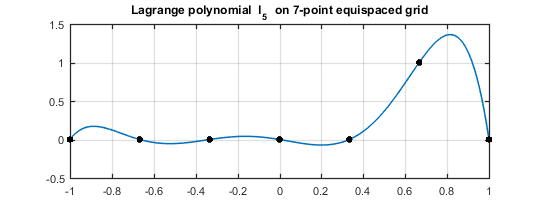
\includegraphics [width=4in]{chap5_01.png}
\begin{par}
 \vskip 1pt 
\end{par} \vspace{1em}
\begin{par}

It is easy to write down an explicit expression for $\ell_j$:
$$ \ell_j(x) = {\prod_{k\ne j} (x-x_k) \over \prod_{k\ne j} (x_j-x_k)}.
\eqno (5.3) $$
Since the denominator is a constant, this function is a polynomial of
degree $n$ with zeros at the right places, and clearly it takes the value
$1$ when $x=x_j$. Equation (5.3) is very well known and can be found in
many textbooks as a standard representation for Lagrange interpolants.
Lagrange worked with (5.1) and (5.3) in 1795 [Lagrange 1795],
and his name is firmly
attached to these ideas,\footnote{Perhaps Cauchy did some of
the attaching, since he wrote in his {\em Cours d'analyse,} ``Cette formule, donn\'ee pour la
premi\`ere fois par Lagrange$,\dots $'' [Cauchy 1821].} but the same formulas were published earlier by
Waring [1779] and Euler [1783], who had been Lagrange's predecessor at
the Berlin Academy.

\end{par} \vspace{1em}
\begin{par}
Computationally speaking, (5.1) is excellent but (5.3) is not so good. It requires $O(n)$ operations to evaluate $\ell_j(x)$ for each value of $x$, and then $O(n)$ such evaluations must be added up in (5.1), giving a total operation count of $O(n^2)$ for evaluating $p(x)$ at a single value of $x$.
\end{par} \vspace{1em}
\begin{par}

By a little rearrangement we can improve the operation count. The key
observation is that for the various values of $j$, the numerators in
(5.3) are the same except that they are missing different factors
$x-x_j$. To take advantage of this commonality, we define the {\em node
polynomial} $\ell\in {\cal P}_{n+1}$ for the given grid by
$$ \ell(x) = \prod_{k=0}^n (x-x_k).  \eqno (5.4) $$
Then (5.3) becomes the elementary but extremely important identity
$$ \ell_j(x) = {\ell(x) \over\ell'(x_j) (x-x_j)}. \eqno (5.5) $$
(We shall use this equation to derive the Hermite integral formula in
Chapter 11.) Equivalently, let us define
$$ \lambda_j = {1\over \prod_{k\ne j} (x_j-x_k)}, \eqno (5.6) $$
that is,
$$ \lambda_j = {1\over \ell'(x_j)} . \eqno (5.7) $$
Then (5.3) becomes
$$ \ell_j(x) = \ell(x) {\lambda_j \over x-x_j}, \eqno (5.8) $$
and the Lagrange formula (5.1) becomes
$$ p(x) = \ell(x) \sum_{j=0}^n {\lambda_j\over x - x_j} \kern 1pt
f_j . \eqno (5.9) $$
These formulas were derived by Jacobi in his PhD thesis in Berlin [Jacobi
1825], and they appeared in 19th century textbooks.\footnote{I am
grateful to Folkmar Bornemann for drawing this history to my attention.}

\end{par} \vspace{1em}
\begin{par}
Equation (5.9) has been called the ``modified Lagrange formula'' (by Higham) and the ``first form of the barycentric interpolation formula'' or the ``type 1 barycentric formula'' (starting with Rutishauser). What is valuable here is that the dependence on $x$ inside the sum is so simple. If the weights $\{\lambda_j\}$ are known, (5.9) produces each value $p(x)$ with just $O(n)$ operations.  Computing the weights from (5.6) requires $O(n^2)$ operations, but this computation only needs to be done once and for all, independently of $x\kern 1pt$; and for special grids $\{x_j\}$ such as Chebyshev, as we shall see in a moment, the weights are known analytically and don't need to be computed at all.  (For Legendre and other grids associated with orthogonal polynomials, the necessary computations can be carried out very fast; see Exercise 5.11 and Theorem 19.6.)
\end{par} \vspace{1em}
\begin{par}

However, there is another barycentric formula that is more elegant. If we
add up all the Lagrange polynomials $\ell_j$, we get a polynomial in
${\cal P}_n$ that takes the value $1$ at every point of the grid.  Since
polynomial interpolants are unique, this must be the constant polynomial
$1$:
$$ \sum_{j=0}^n \ell_j(x) = 1. $$
Dividing (5.8) by this expression enables us to cancel the factor
$\ell(x)$, giving
$$ \ell_j(x)= {\lambda_j \over x-x_j} \left/
        \sum_{k=0}^n{}{\lambda_k \over x-x_k}.\right. \eqno (5.10) $$
By inserting these representations in (5.1), we get the ``second form of
the barycentric interpolation formula'' or ``true barycentric
formula'' for polynomial interpolation in
an arbitrary set of $n+1$ points $\{x_j\}$.

\end{par} \vspace{1em}
\begin{par}
 \em
{\bf Theorem 5.1. Barycentric interpolation formula.}
The polynomial interpolant through data $\{f_j\}$ at $n+1$ points
$\{x_j\}$ is given by
$$ p(x)= \sum_{j=0}^n { \lambda_j f_j \over x-x_j} \left/
        \sum_{j=0}^n{}{\lambda_j \over x-x_j},\right. \eqno (5.11) $$
with the special case $p(x) = f_j$ if $x=x_j$ for some $j$,
where the weights $\{\lambda_j\}$ are defined by
$$ \lambda_j = {1 \over \prod_{k\ne j} (x_j-x_k)} . \eqno (5.12) $$

\end{par} \vspace{1em}
\begin{par}
\textit{Proof.} Given in the discussion above. $~\hbox{\vrule width 2.5pt depth 2.5 pt height 3.5 pt}$
\end{par} \vspace{1em}
\begin{par}
It is obvious that the function defined by (5.11) interpolates the data.  As $x$ approaches one of the values $x_j$, one term in the numerator blows up and so does one term in the denominator. Their ratio is $f_j$, so this is clearly the value approached as $x$ approaches $x_j$.  On the other hand if $x$ is equal to $x_j$, we can't use the formula: that would be a division of $\infty$ by $\infty$.  This is why the theorem is stated with the qualification for the special case $x=x_j$.
\end{par} \vspace{1em}
\begin{par}

What is not obvious is that the function defined by (5.11) is a
polynomial, let alone a polynomial of degree $n$: it looks like a
rational function.  The fact that it is a polynomial depends on
the special values (5.12) of the weights.  For choices of nonzero weights that
differ from (5.12), (5.11) will still interpolate the data, but in
general it will be a rational function that is not a polynomial.   These
rational barycentric interpolants can be very useful in some
applications, and they are likely to get more attention in the future
[Berrut, Baltensperger \& Mittelmann 2005, Tee \& Trefethen 2006, Floater \& Hormann 2007,
Berrut, Floater \& Klein 2011].

\end{par} \vspace{1em}
\begin{par}
Chebfun's overload of the Matlab \texttt{interp1} command, which was illustrated at the beginning of this chapter, incorporates an implementation of (5.11)--(5.12). We shall make use of \texttt{interp1} again in Exercise 5.7 and in Chapters 13 and 15. Now, however, let us turn to the special case that is so important in practice.
\end{par} \vspace{1em}
\begin{par}
For Chebyshev points, the weights $\{\lambda_j\}$ are wonderfully simple: they are equal to $(-1)^j$ times the constant $2^{n-1}/n$, or half this value for $j=0$ and $n$.  These numbers were worked out by Marcel Riesz in 1916 [Riesz 1916]. The constant cancels in the numerator and denominator when we divide by the formula for 1 in (5.11), giving Salzer's amazingly simple result from 1972 [Salzer 1972]:
\end{par} \vspace{1em}
\begin{par}
 \em
{\bf Theorem 5.2. Barycentric interpolation in Chebyshev points.}
The polynomial interpolant through data $\{f_j\}$ at the Chebyshev
points $(2.2)$ is
$$ p(x)=\sum_{j=0}^n{}'{(-1)^j f_j\over x-x_j} \left/
        \sum_{j=0}^n{}'{(-1)^j\over x-x_j},\right. \eqno (5.13) $$
with the special case $p(x) = f_j$ if $x=x_j$. The primes on the
summation signs signify that the terms $j=0$ and $j=n$ are  multiplied by
$1/2$.

\end{par} \vspace{1em}
\begin{par}
Equation (5.13) is scale-invariant: for interpolation in Chebyshev points scaled to any interval $[a,b\kern .3pt]$, the formula is exactly the same. This is a big advantage on the computer when $n$ is in the thousands or higher, because it means that we need not worry about underflow or overflow.
\end{par} \vspace{1em}
\begin{par}

{\em Proof.}
Equation (5.13) is a special case of (5.11).  To prove it, we will show
that for Chebyshev points, the weights (5.12) reduce to $(-1)^j$ times
the constant $2^{n-1}/n$, and half this value for $j=0$ or $n$.
To do this, we begin by noting that for Chebyshev points, the node
polynomial (5.4) can be written as $ \ell(x) = 2^{-n} ( T_{n+1}(x) -
T_{n-1}(x))$ (Exercise 4.1). Together with (5.8), this implies
$$ \ell_j(x) = 2^{-n}\kern 1pt \lambda_j
{T_{n+1}(x) - T_{n-1}(x)\over x-x_j}, $$
and from (5.7) we have
$$ \lambda_j = {1\over \ell'(x_j)} = {2^n\over T_{n+1}'(x_j) - T_{n-1}'(x_j)}. $$
Now it can be shown that
$$ T_{n+1}'(x_j) - T_{n-1}'(x_j) = 2n (-1)^j, \quad 1\le j \le n-1, $$
with twice this value for $j=0$ and $n$ (Exercise 5.3).  So we have
$$ \lambda_j = {2^{n-1}\over n} (-1)^j,  \quad 1\le j \le n-1, \eqno (5.14) $$
with half this value for $j=0$ and $n$, as claimed.
$~\hbox{\vrule width 2.5pt depth 2.5 pt height 3.5 pt}$

\end{par} \vspace{1em}
\begin{par}
The formula (5.13) is extraordinarily effective, even if $n$ is in the thousands or millions, even if $p$ must be evaluated at thousands or millions of points.  As a first example, let us construct a rather wiggly chebfun:
\end{par} \vspace{1em}
\begin{par}
 \vspace{-2em} 
\end{par} \vspace{1em}
\begin{verbatim}
x = chebfun('x');
f = tanh(20*sin(12*x)) + .02*exp(3*x).*sin(300*x);
length(f)
\end{verbatim}

        \color{lightgray} \begin{verbatim}ans =
        5138
\end{verbatim} \color{black}
    \begin{par}
We now plot \texttt{f} using 10000 sample points and note the time required:
\end{par} \vspace{1em}
\begin{par}
 \vspace{-2em} 
\end{par} \vspace{1em}
\begin{verbatim}
hold off
tic, plot(f,'linewidth',.5,'numpts',10000), toc
title('A rather wiggly function',FS,9)
\end{verbatim}

        \color{lightgray} \begin{verbatim}Elapsed time is 0.056949 seconds.
\end{verbatim} \color{black}
    
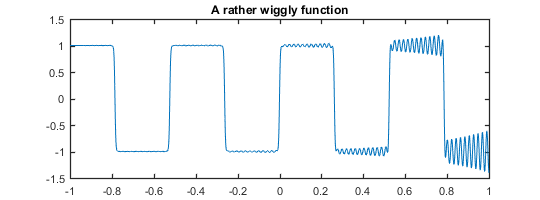
\includegraphics [width=4in]{chap5_02.png}
\begin{par}
 \vskip 1pt 
\end{par} \vspace{1em}
\begin{par}
In this short time, Chebfun has evaluated a polynomial interpolant of degree about 5000 at 10000 sample points.
\end{par} \vspace{1em}
\begin{par}
Raising the degree further, let $p$ be the Chebyshev interpolant of degree $10^6$ to the function $\sin(10^5 x)$ on $[-1,1]$:
\end{par} \vspace{1em}
\begin{par}
 \vskip -2em 
\end{par} \vspace{1em}
\begin{verbatim}
ff = @(x) sin(1e5*x); p = chebfun(ff,1000001);
\end{verbatim}
\begin{par}
How long does it take to evaluate this interpolant at 100 points?
\end{par} \vspace{1em}
\begin{par}
 \vskip -2em 
\end{par} \vspace{1em}
\begin{verbatim}
xx = linspace(0,0.0001); tic, pp = p(xx); toc
\end{verbatim}

        \color{lightgray} \begin{verbatim}Elapsed time is 0.235412 seconds.
\end{verbatim} \color{black}
    \begin{par}
Not bad for a million-degree polynomial!  The result looks fine,
\end{par} \vspace{1em}
\begin{par}
 \vskip -2em 
\end{par} \vspace{1em}
\begin{verbatim}
clf, plot(xx,pp,'.','markersize',10), axis([0 0.0001 -1 1])
title('A polynomial of degree 10^6 evaluated at 100 points',FS,9)
\end{verbatim}

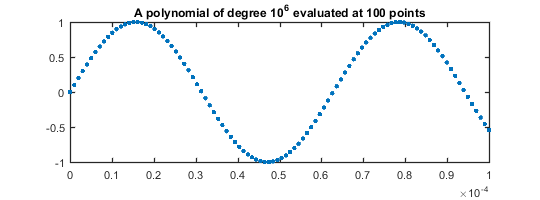
\includegraphics [width=4in]{chap5_03.png}
\begin{par}
 \vskip -10pt 
\end{par} \vspace{1em}
\begin{par}

\noindent and it matches the target function closely:

\end{par} \vspace{1em}
\begin{par}
 \vskip -2em 
\end{par} \vspace{1em}
\begin{verbatim}
format long
for j = 1:5
    r = rand; disp([ff(r) p(r) ff(r)-p(r)])
end
\end{verbatim}

        \color{lightgray} \begin{verbatim}   0.705930356624765   0.705930356611629   0.000000000013136
  -0.931512002954607  -0.931512002956252   0.000000000001645
   0.583585101736752   0.583585101731217   0.000000000005535
  -0.851482366899905  -0.851482366905168   0.000000000005262
   0.988082673530624   0.988082673531113  -0.000000000000489
\end{verbatim} \color{black}
    \begin{par}
The apparent loss of 4 or 5 digits of accuracy is to be expected since the derivative of this function is of order $10^5$: each evaluation is the correct result for a value of $x$ within about $10^{-16}$ of the correct one (Exercise 5.5).
\end{par} \vspace{1em}
\begin{par}
Experiments like these show that barycentric interpolation in Chebyshev points is a robust process: it is numerically stable, untroubled by rounding errors on a computer. This may seem surprising if you look at (5.9) or (5.13)---shouldn't cancellation errors on a computer cause trouble if $x$ is close to one of the Chebyshev points $x_j$? In fact they do not, and these formulas have been proved stable in floating point arithmetic for all $x\in[-1,1]$ [Rack \& Reimer 1982, Higham 2004]. This is in marked contrast to the more familiar algorithm of polynomial interpolation via solution of a Vandermonde linear system of equations, which is exponentially unstable (Exercise 5.2).
\end{par} \vspace{1em}
\begin{par}

We must emphasize that whereas (5.13) is stable for interpolation,
it is unstable for extrapolation, that is, the evaluation of $p(x)$
for $x\not\in [-1,1]$.  The more general formula (5.11) is unstable for
extrapolation too and is unstable even for
interpolation when used with arbitrary points rather than points
suitably clustered like Chebyshev points.  In these cases it is
important to use the ``type 1'' barycentric formula (5.9) instead,
which Higham proved stable in all cases.  The disadvantage of (5.9)
is that when $n$ is larger than about a thousand, it is susceptible
to troubles of underflow or overflow, which must be countered by
rescaling $[-1,1]$ to $[-2,2]$ or by computing products by addition
of logarithms.

\end{par} \vspace{1em}
\begin{par}
More precisely, Higham [2004] showed that when they are used to evaluate $p(x)$ for $x\in [-1,1]$ with data at Chebyshev points, both (5.9) and (5.11)--(5.13) have a certain property that numerical analysts call \textit{forward stability}. If you want to evaluate $p(x)$ for values of $x$ outside $[-1,1]$, however, (5.11)--(5.13) lose their stability and it is important to use (5.9), which has the stronger property known as \textit{backward stability} [Webb, Trefethen \& Gonnet 2011]. It is also important to use (5.9) rather than (5.11) for computing interpolants through equispaced points or other point sets that are far from the Chebyshev distribution. (As we shall discuss in Chapters 13--14, in these cases the problem is probably so ill-conditioned that one should not be doing polynomial interpolation in the first place.)
\end{par} \vspace{1em}
\begin{par}
These observations show that (5.9) has advantages over (5.11) and (5.13), but it also has an important disadvantage: it is not scale-invariant, and the weights grow exponentially as functions of the inverse of the length of the interval of interpolation. We see this in (5.14), where the weights have size $2^n$, and would in fact overflow on a computer in standard IEEE double precision arithmetic for $n$ bigger than about 1000. (Higham's analysis ignores overflow and underflow.) We shall have more to say about this exponential dependence in Chapters 11--15. So (5.11) and (5.13) remain a good choice for most applications, so long as the interpolation points are Chebyshev or similar and the evaluation points lie in $[-1,1]$.
\end{par} \vspace{1em}
\begin{par}

\begin{displaymath}
\framebox[4.7in][c]{\parbox{4.5in}{\vspace{2pt}\sl
{\sc Summary of Chapter 5.}
Polynomial interpolants can be evaluated fast and stably by
the barycentric formula, even for thousands or millions of interpolation
points.  The barycentric formula has the form of a rational function, but
reduces to a polynomial because of the use of specially determined
weights.\vspace{2pt}}}
\end{displaymath}

\end{par} \vspace{1em}
\begin{par}
 \smallskip\small\parskip=2pt
{\bf Exercise 5.1.  Barycentric coefficients by hand.} (a) Work out on
paper the barycentric interpolation coefficients $\{\lambda_j\}$ for the
case $n=3$ and $x_0 = -1$, $x_1 = 0$, $x_2 = 1/2$, $x_3 = 1$.  (b)
Confirm that (5.9) gives the right value $p(-1/2)$ for the polynomial
interpolant to data $1,2,3,4$ in these points.
\par
{\bf Exercise 5.2.  Instability of Vandermonde interpolation.} The
best-known numerical algorithm for polynomial interpolation, unlike the
barycentric formula, is unstable.  This is the method implemented in the
Matlab {\tt polyfit} command, which forms a Vandermonde matrix of sampled
powers of $x$ and solves a corresponding linear system of equations.  (In
[Trefethen 2000], to my embarrassment, this unstable method is used
throughout, forcing the values of $n$ used for plots in that book to be
kept small.)  (a) Explore this instability by comparing a Chebfun
evaluation of $p(0)$ with the result of {\tt polyval(polyfit({\tt
xx},f({\tt xx}),n),0)} where {\tt f = @(x) cos(k*x)} for $k = 10,
20,\dots, 90, 100$, $n$ is the degree of the corresponding chebfun, and
{\tt xx} is a fine grid. (b) Examining the Matlab {\tt polyfit} code as
appropriate, construct the Vandermonde matrices $V$ for each of these ten
problems and compute their condition numbers.  (You can also use the
Matlab {\tt vander} command.)  By contrast, the underlying Chebyshev
interpolation problem is well-conditioned.
\par
{\bf Exercise 5.3.  Calculating derivatives for the proof of Theorem 5.2.}
Derive the following identities used in the proof of Theorem 5.2.
(a) For $1 \le j \le n-1$, $T_{n+1}'(x_j) - T_{n-1}'(x_j) = 2n (-1)^j$.
(b) For $j = 0$ and $j=n$, $T_{n+1}'(x_j) - T_{n-1}'(x_j) = 4n (-1)^j$.
One can derive this formula directly, or indirectly by a symmetry
argument.
\par
{\bf Exercise 5.4.  Interpolating the sign function.}
Use {\tt x = chebfun('x')}, {\tt f = sign(x)} to construct the sign
function on $[-1,1]$ and {\tt p = chebfun('sign(x)',10000)} to construct
its interpolant in 10000 Chebyshev points.  Explore the difference in the
interesting region by defining {\tt d = f-p}, \verb|d = d{-0.002,0.002}|.
What is the maximum value of {\tt p}? In what subset of $[-1,1]$ is {\tt
p} smaller than $0.5$ in absolute value?
\par
{\bf Exercise 5.5.  Accuracy of point evaluations.}
(a) Construct the chebfun $g$ corresponding to $f(x) = \sin(\exp(10 x))$
on $[-1,1]$.  What is the degree of this polynomial? (b) Let {\tt xx} be
the vector of 1000 linearly spaced points from $-1$ to $1$.  How long
does it take on your computer to evaluate $f({\tt xx})$?  $g({\tt xx})$?
(c) Draw a loglog plot of the vector of errors $|f({\tt xx}) - g({\tt
xx})|$ against the vector of derivatives $|f'({\tt xx})|$.  Comment on
why the dots line up as they do.
\par
{\bf Exercise 5.6.  Equispaced points.}
Show that for equispaced points in $[-1,1]$ with spacing
$h$, the barycentric weights are $\lambda_j = (-1)^{n-j}/
(\kern .7pt j! \kern .7pt (n-j)!\kern .7pt h^n)$,
or after canceling common factors, $\lambda_j = (-1)^j {n \choose j}$
[Taylor 1945].
\par
{\bf Exercise 5.7.  A greedy algorithm for choosing interpolation grids.}  Write a program
using Chebfun's \verb|interp1| command to compute a sequence of polynomial
interpolants to a function
$f$ on $[-1,1]$ in points selected by a greedy
algorithm: take $x_0$ to be a point where $|f(x)|$ achieves its maximum,
then $x_1$ to be a point where $|(f-p_0)(x)|$ achieves its maximum,
then $x_2$ to be a point where $|(f-p_1)(x)|$ achieves its maximum,
and so on. Plot the error curves $(f-p_n)(x)$, $x\in [-1,1]$ computed
by this algorithm for $f(x) = |x|$ and $0\le n \le 25$.  Comment on the
spacing of the grid $\{x_0,\dots,x_{25}\}$.
\par
{\bf Exercise 5.8.  Barycentric formula for Chebyshev polynomials.}
Derive an elegant formula for $T_n(x)$ from (5.13) [Salzer 1972].
\par
{\bf Exercise 5.9.  Barycentric interpolation in roots of unity.}
Derive the barycentric weights $\{\lambda_j\}$ for polynomial
interpolation in (a) $\{\pm 1\}$, (b) $\{1, i, -1, -i\}$,
(c) The $(n+1)$st roots of unity for arbitrary $n\ge 0$.
\par
{\bf Exercise 5.10.  Barycentric weights for a general interval.}
(a) How does the formula (5.14) for Chebyshev barycentric weights on $[-1,1]$
change for weights on an interval $[a,b\kern .3pt]$?  (b) The {\em capacity} of
$[a,b\kern .3pt]$ (see Chapter 12) is equal to $c = (b-a)/4$.  How do the
barycentric weights behave as $n\to\infty$ for an interval of capacity
$c$? As a function of $c$, what is the maximal value of $n$ for which
they can be represented in IEEE double precision arithmetic without
overflow or underflow?  (You may assume the overflow and underflow limits
are $10^{308}$ and $10^{-308}$. The overflow/underflow problem goes away
with the use of the divided form (5.13).)
\par
{\bf Exercise 5.11.  Barycentric interpolation in Legendre points.}
Chebfun includes fast
algorithms for computing barycentric weights for various distributions
of points other than Chebyshev, such as Legendre points, the zeros
of Legendre polynomials (see Chapter 17 and Theorem 19.6).  Perform a
numerical experiment to compare
the accuracy of interpolants in Chebyshev and Legendre points to
$f(x) = e^x \sin(300x)$ at $x=0.99$.  Specifically,
compute \verb|[s,w,lambda] = legpts(n+1)| and
\verb|bary(0.99,f(s),s,lambda)| for $1\le n \le 500$ and make a semilog
plot of the absolute value of the error as a function of $n$;
compare this with the analogous plot for Chebyshev points.
\par
{\bf Exercise 5.12.  Barycentric rational interpolation.}
(a) If the formula (5.13) is used with points $\{x_j\}$ other than
Chebyshev with maximum spacing $h$, it produces a
rational interpolant of accuracy $O(h^2)$ as $h\to0$ [Berrut 1988].
Confirm this numerically for $f(x) = e^x$ and equispaced points
in $[-1,1]$.  (b) Show numerically that the accuracy improves
to $O(h^3)$ if the pattern of coefficients near the left end
is changed from $\textstyle{1\over 2}, -1, 1, -1, \dots$ to
$\textstyle{1\over 4}, -\textstyle{3\over 4}, 1, -1, \dots$
and analogously at the right end [Floater \& Hormann 2007].
\par
{\bf Exercise 5.13.  Barycentric weights and geometric mean distances.}
(a) Give an interpretation of (5.6) in terms of geometric mean
distances between grid points.  (b) Explain how one of the theorems
of this chapter explains the result of Exercise 2.6.
\par 
\end{par} \vspace{1em}



\end{document}
    
